\chapter*{Introduction}
\addcontentsline{toc}{chapter}{Introduction}
\markboth{}{}
\label{chap:intro}
In this work we consider cooperative multi-agent scenarios, in which multiple 
robots collaborate, and possibly communicate, to achieve a common goal 
\cite[][]{ismail2018survey}.
Homogeneous Multi-Agent Systems (MAS) are composed of $N$ interacting 
agents, which have the same physical structure and observation capabilities, so 
they can be considered to be interchangeable and cooperate to solve a given 
task \cite[][]{stone2000multiagent, vsovsic2016inverse}.
This system is characterised by a state $S$ — which can be decomposed in sets of 
local states for each agent and the set of possible observations $O$ for each agent 
— obtained through sensors and the set of possible actions  $A$ for each agent.

The objective of this study is to use \gls{il} approaches to learn decentralised 
solutions via imitation of an omniscient centralised control. To do so we train 
end-to-end \glspl{nn}, either classifiers or regressors, that only exploit local 
observations and communications to decide the action to be performed. This 
controller is the same for each agent, which means that given an identical set of 
observations as input, likewise, for each of these the outputs will be equivalent 
\cite[][]{ross2011reduction, tolstaya2020learning}.

This research project focuses on two different multi-agent scenarios, in which $N$ 
robots, all oriented in the same direction, are initially randomly placed along the 
$x$-axis. We consider the Thymio as holonomic, since their movements are 
limited in only one dimension. This premise simplifies our system, in which 
consequently we have to keep into account only geometric constraints and not 
kinematic.

In the first scenario, visualised in Figure \ref{fig:task1}, the objective is to 
distribute the robots in space such that they stand at equal distance from each 
other. To do so, each agent updates its state — its absolute position — by 
performing actions — moving forward and backwards along the $x$-axis — 
based on the observations received from the environment — the distances from 
neighbours.
\begin{figure}[!htb]
	\begin{center}
		\begin{subfigure}[h]{0.49\textwidth}
		\centering
		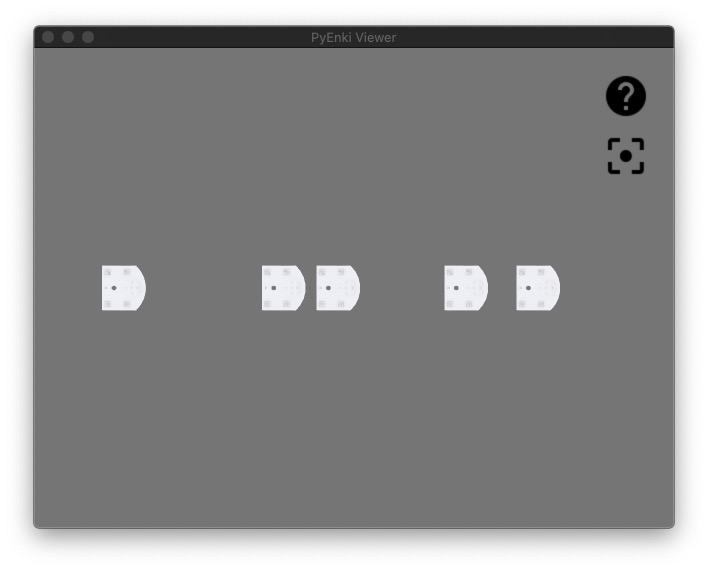
\includegraphics[width=\textwidth]{contents/images/task1init}
		\end{subfigure}
		\hfill
		\begin{subfigure}[h]{0.49\textwidth}
			\centering
			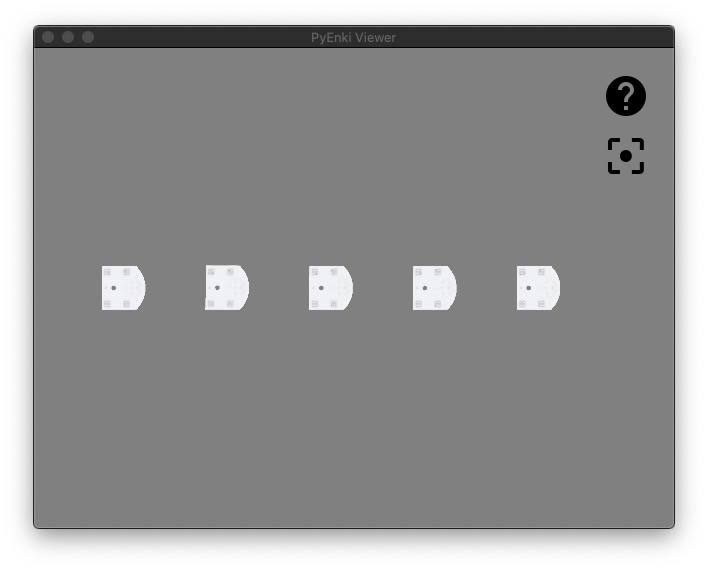
\includegraphics[width=\textwidth]{contents/images/task1final}
		\end{subfigure}
	\end{center}
	\vspace{-0.5cm}
	\caption[Visualisation of the simulation of the first task.]{Visualisation of the 
	initial and final configurations obtained simulating the first task.}
	\label{fig:task1}
%	\vspace{-0.5cm}
\end{figure}
Perceiving the environment using its own sensors, in particular sensing the 
distances from the neighbours, each robot achieves the goal moving towards the 
target by minimising the difference between the values recorded by the front and 
rear sensors, trying to maintain the maximum achievable speed. This means that 
each robot is at the same distance from the one in front and the one behind, that 
should be the same distance among all the agents.

\bigskip
In the second scenario, shown in Figure \ref{fig:task2}, assuming that the agents 
in space are divided into two sets, the objective is to colour them depending on 
their group membership. 
For the sake of simplicity, we decide the group each robot belongs to based on 
the total number of robots: in case of an even number of agents, those in the first 
half of the row belong to the first group and the remaining to the second, while in 
the case of an odd number of robots, the same reasoning is applied and the 
central agent is assigned to the first set.
To perform this task, each agent performs actions — colouring the top \gls{led} 
in red or blue — based on the observations received from the environment — the 
messages received from neighbours. 
\begin{figure}[!htb]
	\begin{center}
		\begin{subfigure}[h]{0.49\textwidth}
			\centering
			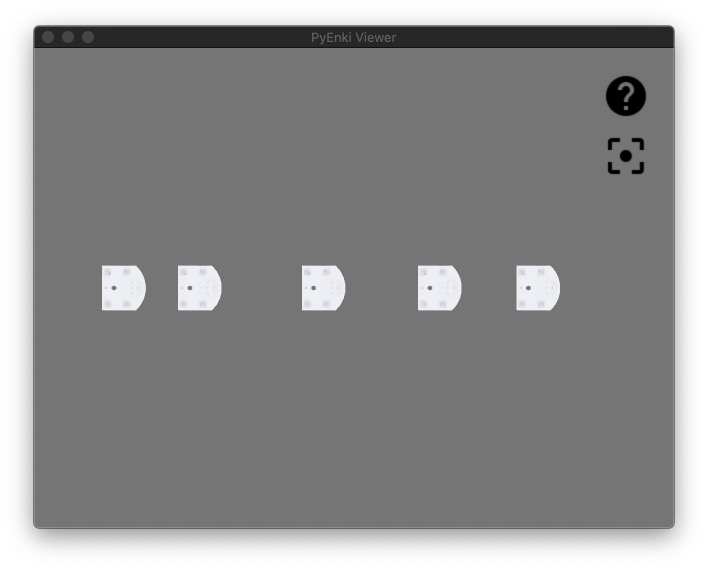
\includegraphics[width=\textwidth]{contents/images/task2init}
		\end{subfigure}
		\hfill
		\begin{subfigure}[h]{0.49\textwidth}
			\centering
			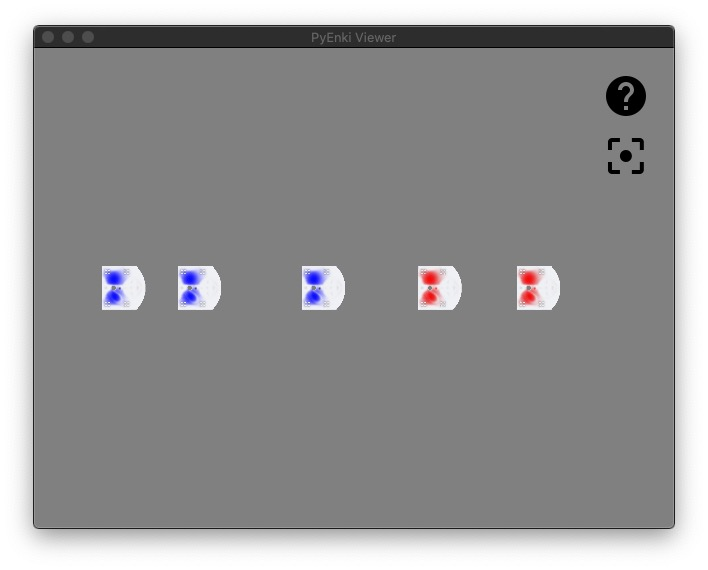
\includegraphics[width=\textwidth]{contents/images/task2final}
		\end{subfigure}
	\end{center}
	\vspace{-0.5cm}
	\caption[Visualisation of the simulation of the second task.]{Visualisation of the 
		initial and final configurations obtained simulating the second task.}
	\label{fig:task2}
\end{figure}
This time, sensing the distance from neighbours does not provide useful 
information about the order of the agents, therefore they are not considered to 
accomplish this task. Instead, the only way for the robots to understand their 
ordering is necessarily using a communication protocol. For example, starting 
from the extreme agents, the first and the last in the row, or those that cannot 
receive any communication respectively from back and front, all the robots 
retransmit the received value, increased by one. In this way, the agents will in a 
sense, learn to count in order to understand which is the correct value to transmit.

Both the scenarios are examples of cooperative tasks based on the use of a 
distributed controller. While the second cannot be solved without allowing an 
explicit exchange of messages between the agents, in the first one a 
communication protocol is not necessary, but it may nonetheless increase 
performance.
To solve these tasks we have adopted two different methodologies, depending on 
whether the communication is used or not.
First of all, we analyse typical supervised learning approaches, which directly learn 
a mapping from observations to actions. This method can be applied only to the 
first task, in which a very simple ``distributed network'' that takes as input an 
array containing the response values of the sensors — either 
\texttt{prox\_values},  \texttt{prox\_comm} or  \texttt{all\_sensors} — and 
produces as output an array containing one float that represents the speed of the 
wheels, which is assumed to be the same both right and left, so that the robot 
moves straight.
After that, we concentrate on more challenging situations where the 
communication is not provided to the network, instead, it is a latent variable 
which has to be inferred \cite[][]{le2017coordinated}.
Throughout the experiments, we show the effectiveness of our methods, 
comparing approaches with and without communication. We also analyse the 
effects of varying the inputs of the networks, the initial distance between the 
robot and the number of agents chosen.

\subsubsection*{Outline}
\label{subsec:outline}

The thesis is composed of 6 chapters, whose main points are presented as follows:
\begin{itemize}
	\item Chapter \ref{chap:stateoftheart} summarises the previous research 
	on the topic, evaluating the approaches adopted by the authors;
	
	\item Chapter \ref{chap:background} provides the background knowledge 
	needed to properly understand the research contents;
	
	\item Chapter \ref{chap:impl} presents the tools used for the data collection 
	and all the additional frameworks we relied on;
		
	\item Chapter \ref{chap:methods} thoroughly illustrates the methodology used, 
	their benefits and limitations, also including descriptions of the kind of data 
	used and how they are collected;

	\item Chapter \ref{chap:experiments} explores the analysis conducted and 
	shows evaluation results;	
	
	\item The \hyperref[chap:concl]{Conclusion} addresses the results of the 
	experiments, concludes the thesis by discussing the implications of our findings, 
	possible improvements and outlines future works.
	
\end{itemize}

